\subsection{Temps}
\label{section:work:time}

Pour pouvoir maintenir notre environnement virtuel, nous avons expliqué en section \ref{subsubsection:time} que nous ne pouvons pas laisser les applications accéder aux horloges de la machine hôte, utilisant pour cela la bibliothèque \texttt{VDSO}. Nous avons alors proposé de créer une bibliothèque réimplémentant les fonctions temporelles et d'utiliser la variable d'envieronnement \texttt{LD\_PRELOAD}, présentée en section \ref{paragraphe:LDPreload}, pour exécuter les fonctions de notre bibliothèque en priorité. De cette façon, on bloque les appels à la bibliothèque \texttt{VDSO} et l'application ne peut plus accéder au temps de la machine hôte. Néanmoins, pour que notre virtualisation soit parfaite il faudrait que le temps que l'applicatioin voit s'écouler soit celui qui s'écoulerait sur la machine simulée par SimGrid. 

Pour permettre cela, nous avons créé une bibliothèque de fonctions temporelles que nous plaçons dans la variable d'environnement \texttt{LD\_PRELOAD} à chaque exécution d'une application avec Simterpose. Cette bibliothèque contient pour chaque fonction de la \texttt{libc} qui fasse appel à une des horloges de la machine (\texttt{ftime}, \texttt{time}...) une nouvelle fonction de même prototype. Maintenant, au lieu de demander l'horloge de la machine hôte, les nouvelles fonctions de temps demandent à SimGrid de fournir l'heure sur la machine qu'il est en train de simuler. Comme le montre la figure \ref{time_interception}, l'appel à la fonction de temps se fait dans l'application qui s'exécute sur le thread "espionné" de Simterpose. Ce dernier est controlé par le processus 'espion' via l'intercepteur \texttt{ptrace} qui est le seul processus de Simterpose à pouvoir communiquer avec le simulateur. Nous devons donc passer par le thread "espion" pour pouvoir interrroger SimGrid. 

{\color{red} pas clair}
\textit{Cependant, le seul moyen de faire intervenir le processus "espion" est d'effectuer un appel système dans l'application en train de s'exécuter. Dans notre cas, c'est la nouvelle fonction temporelle qui doit effecteur l'appel système. En effet, le processus "espion" va intercepter l'appel et exécuter le "handler" qu'on lui aura fourni si nécessaire, comme pour le reseau de communications, avant de rendre la main à l'application en plaçant dans le registre de retour de l'appel système l'horloge que lui aura donné le simulateur. Si une autre fonction effectue l'appel, la nouvelle fonction temporelle ne pourra pas récupérer la valeur de retour de l'appel système et ainsi retourner l'heure simulée à l'application. De plus, puisque nous souhaitons juste récupérer l'horloge de l'environnement virtuel et rien d'autre, il faudra que le "handler" que va exécuter \texttt{ptrace} avant l'appel contienne l'appel à la fonction \texttt{MSG\_get\_clock}, qui permet de récupérer l'heure dans SimGrid et neutralise l'appel système choisit avant de rendre la main à l'application. 
}

Néanmoins, la fonction temporelle ne doit pas utiliser n'importe quel appel système pour récupérer l'heure simulée. Par exemple, si on choisit de modifier l'appel système \texttt{send}, on va placer dans le handler de ce dernier l'appel à la fonction \texttt{MSG\_get\_clock} puis on le neutralise. Or, lorsqu'on voudra utiliser cet appel système pour envoyer des données sur le réseaux on ne pourra plus le faire car l'intercepteur \texttt{ptrace} exécutera le nouveau handler et l'appel ne sera plus exécuté. Il nous faut donc trouver un appel système dont on n'aura jamais besoin pour faire autre chose que récupérer l'heure simulée. Dans tous les noyaux, il existe des appels systèmes qui ne sont plus implémentés; c'est le cas de l'appel système \texttt{tuxcall}. Quand on fait appel à ce dernier le système ne fait rien, il émet juste un avertissement pour dire que l'appel n'existe plus. De plus, comme cet appel ne produit aucun action de la part du système il n'est pas nécessaire de le neutraliser. Nous avons donc choisi de placer notre handler sur cet appel système.

Les Algorithmes \ref{ALGO_TIME} et \ref{ALGO_TUXCALL} ainsi que la Figure \ref{time_interception} nous montrent respectivement l'algorithme de la nouvelle fonction \texttt{time}, le handler de l'appel système \texttt{tuxcall}, et ce qui se passe dans SimGrid et Simterpose quand on veut récupérer l'heure simulée grâce à la double interception complémentaire de \texttt{LD\_PRELOAD} et \texttt{ptrace}.

\begin{figure}[H]
  \centering
  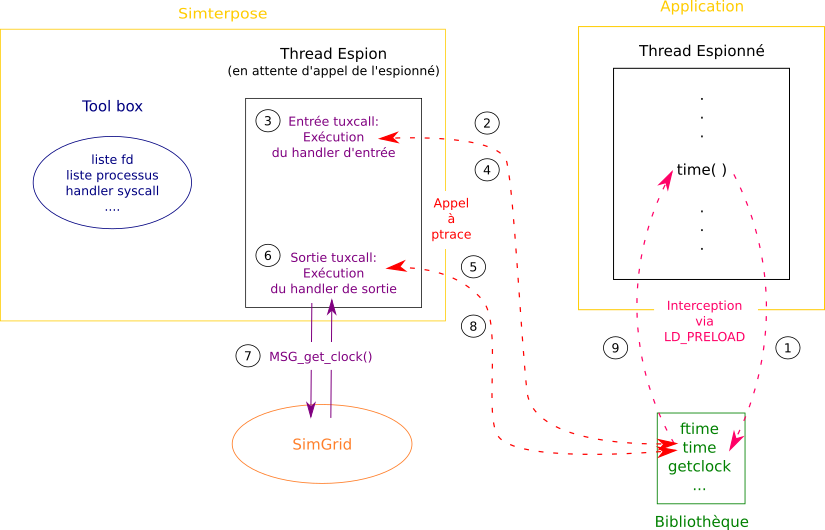
\includegraphics[scale=0.7]{Pictures/png/Open_pandor}
  \caption{Déroulement de l'appel à une fonction temporelle réimplémentée, time dans ce cas}
  \label{time_interception}
\end{figure}

\vspace{2cm}
\lstdefinestyle{customc}{
  belowcaptionskip=1\baselineskip,
  breaklines=true,
   frame=L,
  %%frame=single,
  xleftmargin=\parindent,
  language=C,
  showstringspaces=false,
  basicstyle=\footnotesize\ttfamily,
  keywordstyle=\bfseries\color{blue},
  commentstyle=\itshape\color{green!40!black},
  %%identifierstyle=\color{blue},
  stringstyle=\color{violet},
}
\lstset{escapechar=@,style=customc, caption={Fontion \texttt{time} et appel à \texttt{tuxcall}}, label=ALGO_TIME, captionpos=b}
\begin{lstlisting}
  /* Macro to ask the clock to SimGrid */
  #define get_simulation_time(clock) \
  syscall(SYS_tuxcall, clock); \
  fprintf(stderr, "[%d] get_simulation_time %lfsec\n", getpid(), *sec)

    /* Time function */
    time_t time(time_t *t){
      LogWrap("time call\n");
      double* sec = (double *) malloc(sizeof(double));
      get_simulation_time(sec);
      if (t != NULL)
      t = (time_t *) sec;
      LogWrap("time call done \n");  
      return (time_t)(*sec);    
    }
\end{lstlisting}

\newpage
\lstset{escapechar=@,style=customc, caption={Handler pour l'appel système \texttt{tuxcall}}, label=ALGO_TUXCALL, captionpos=b}
\begin{lstlisting}
  void syscall_tuxcall(reg_s * reg, process_descriptor_t * proc){

  if (proc_entering(proc))
    proc_inside(proc); /* syscall_tuxcall_enter */
  else
    syscall_tuxcall_post(reg, proc);  /* syscall_tuxcall_exit */
  
}

void syscall_tuxcall_post(reg_s * reg, process_descriptor_t * proc){

  proc_outside(proc);
  XBT_DEBUG("tuxcall_post");

  /* Ask the clock to SimGrid */
  double clock = MSG_get_clock();
  
  /* Put the return value in argument register of the syscall */
  /* Uses ptrace because the call in the memory area of another process */
  /* You can access register directly */
  ptrace_poke(proc->pid, (void *) reg->arg[1], &clock, sizeof(double)); 

  if (strace_option)
    print_tuxcall_syscall(reg, proc);
}
\end{lstlisting}

